\chapter{Theoretical background}

This chapter explores three key concepts that power the learning platform: spaced repetition algorithm, Large Language Models and the REST (REpresentational State Transfer). Spaced repetition is a learning technique, that can help improve long-term retention by scheduling the learning material with increasing intervals. It is an evidence-based technique and is usually performed with flashcard-like methods, which makes it practical to implement into the learning platform. On the other hand, LLMs act as knowledge bases that generate targeted questions.

REST is an architectural style for distributed hypermedia systems, originally introduced by Roy Fielding \cite{fielding2000} in his 2000 doctoral dissertation. Despite its widespread adoption in modern web development, it is worth exploring in detail here, particularly focusing on HATEOAS (Hypermedia as the Engine of Application State) - a less commonly understood principle that forms a crucial foundation for a concept discussed later in this thesis. By combining these techniques, the platform can create a tailored learning experience.

\section{Spaced Repetition}

Spaced repetition is a method of learning at semantic intervals. These intervals become longer as the studying process goes on. Initially, these intervals are short, usually a few hours long, and for a long time, they could even be multiple years long. The method's primary goal is to help the practitioner retain the information in long-term memory.

This method is the complete opposite of cramming; it is not trying to learn everything in the shortest possible time. It focuses on understanding the learning material for the long term by "re-learning" it repeatedly after increasing intervals. A German psychologist, Hermann Ebbinghaus, first described this learning technique in the late 19th century. In 1885, He published his research about memory and forgetting in his book On Memory~\cite{ebbinghaus1964memory}.

In his book, He wrote about the \texttt{forgetting curve}, the idea of forgetting information at a predictable rate. He discovered humans forget information rapidly faster after the first learning, but reviewing the information at strategic intervals helps slow down it. The practical application of his theories was developed much later by German science journalist Sebastian Leitner in the 1970s. Figure~\ref{fig:forgetting-curve} visually shows the concept of \texttt{forgetting curve}.

\begin{figure}[!h]
  \centering
  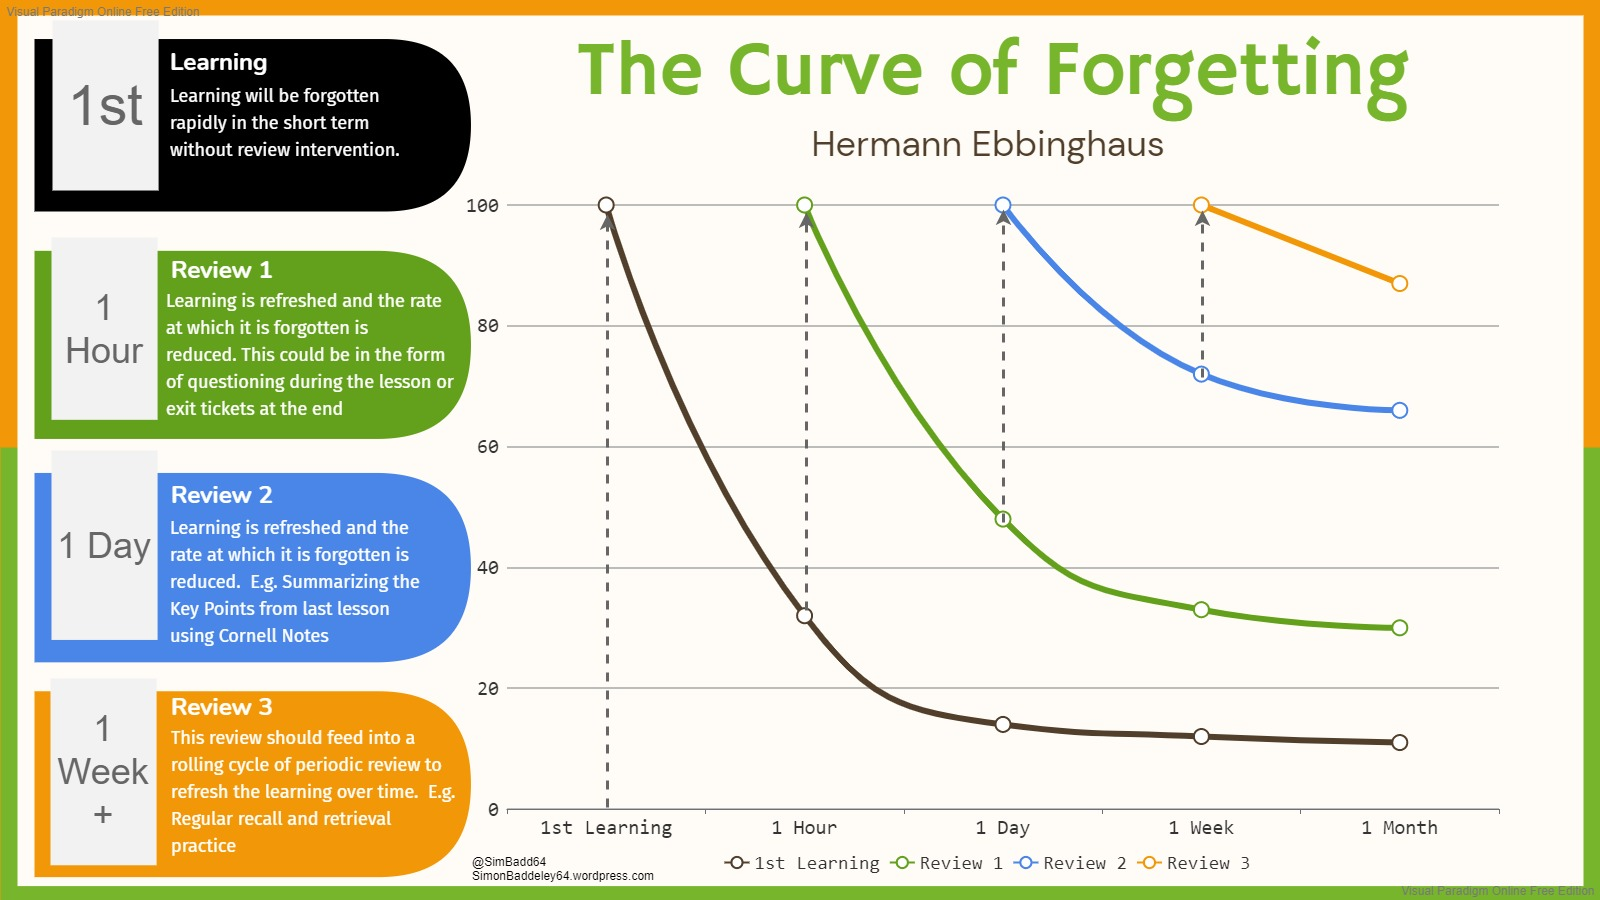
\includegraphics[width=0.8\textwidth, keepaspectratio]{figures/forgetting_curve}
  \caption{The Curve of Forgetting, created by: Simon Baddeley}
  \label{fig:forgetting-curve}
\end{figure}

Leitner's implementation is called the Leitner system \footnote{https://en.wikipedia.org/wiki/Leitner_system}. It is a paper-based method of using flashcards organized into numbered paper boxes. These paper boxes represent review intervals. When a question is answered correctly, it goes up by one, and when answered incorrectly, it goes down by one. Figure~\ref{fig:leitner-system} shows it visually.

\begin{figure}[!h]
  \centering
  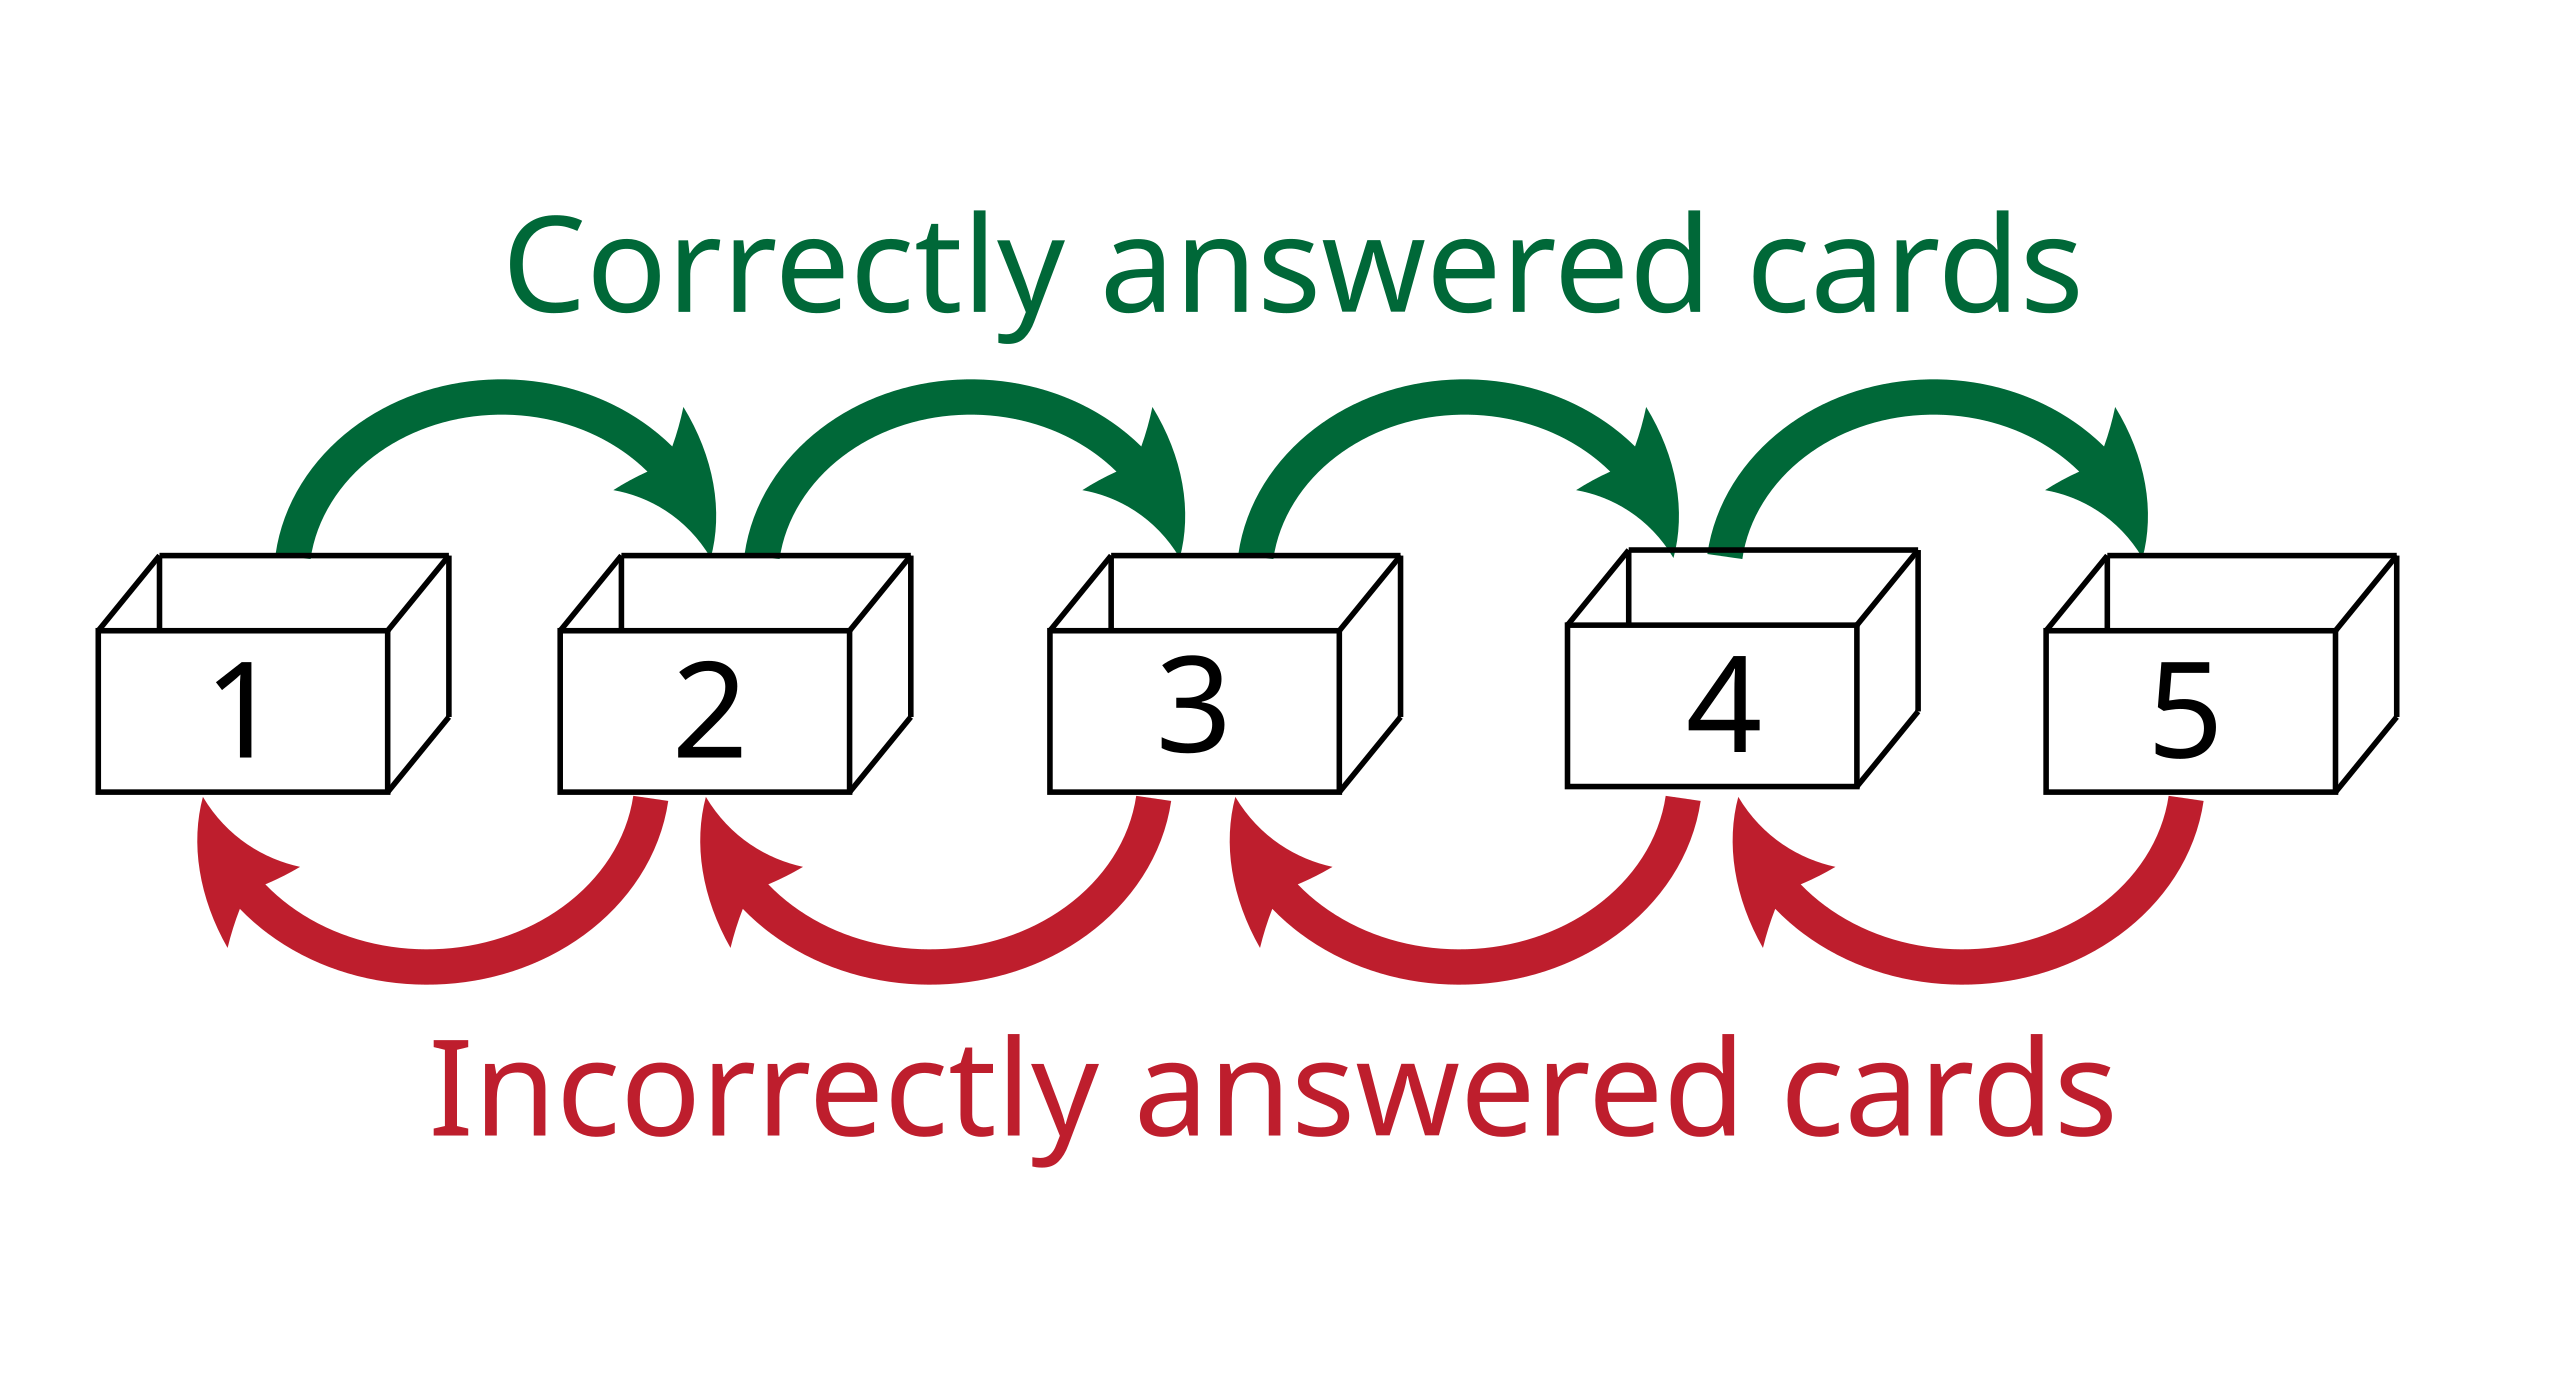
\includegraphics[width=0.8\textwidth, keepaspectratio]{figures/Leitner_system}
  \caption{Leitner system, source: Wikipédia}
  \label{fig:leitner-system}
\end{figure}

In 1987, a Polish computer engineer, Piotr Wozniak, created the first educational software implementing spaced repetition, called \texttt{SuperMemo} \footnote{https://www.supermemo.com/en}. His \texttt{SuperMemo} algorithm calculates the optimum interval for learning. The algorithm has evolved several times over the years; it uses different metrics and parameters to determine the optimal interval. The current version of his algorithm is SM-17\footnote{https://supermemo.guru/wiki/Algorithm_SM-17}. For the platform, I implemented a prototype algorithm similar but simpler to his using similar parameters.

The core parameters of my algorithm are the following: \textt{score}, \textt{difficulty}, \textt{streak}, \textt{interval} and \textt{ease factor}.

\textbf{score}: The \texttt{score} is the score the user reached when answering the given question. It is a number between one and five.

\textbf{difficulty}: The \texttt{difficulty} of the question represents how challenging it is to remember the particular answer. It is used to adjust the review interval.

\textbf{streak}: The \texttt{streak} represents the number of succesful consecutive recalls. It resets to 0 when the user struggles to answer correctly.

\textbf{interval}: The \texttt{interval} is the time between the reviews. It is calculated all the other from all the parameters. It increases exponentially based on user performance.

\textbf{ease factor}: The \texttt{ease factor} measures how easily and item is remembered over time. It increases for good performance and decreases for poor performance.

The concrete Go implementation is detailed at the \texttt{Spaced repetition algorithm} subchapter~\ref{subsec:spaced-repetition-algorithm}.

\section{Large Language Models}
TODO - What is a large language model, how do they work briefly, supervised finetuning, qlora, prompt engineering, dataset, wikipedia articles, the final model(s), how we integrated it to the platform. This is mostly Máté's topic so when he is done i will start to write this part

\section{REST}

The REST architectural style has six guiding principles, all of which must be satisfied by a REST-ful service. Roy names them \cite[Chapter 5]{fielding2000}: Client-Server, Stateless, Cache, Uniform interface, Layered system, and Code-On-Demand.

\subsection{Client-Server}

The Client-Server is the most fundamental architectural style in network-based applications. It consists of two primary components: clients and servers, each with distinct responsibilities, as illustrated in Figure ~\ref{fig:client-server}.

\begin{figure}[!h]
\centering
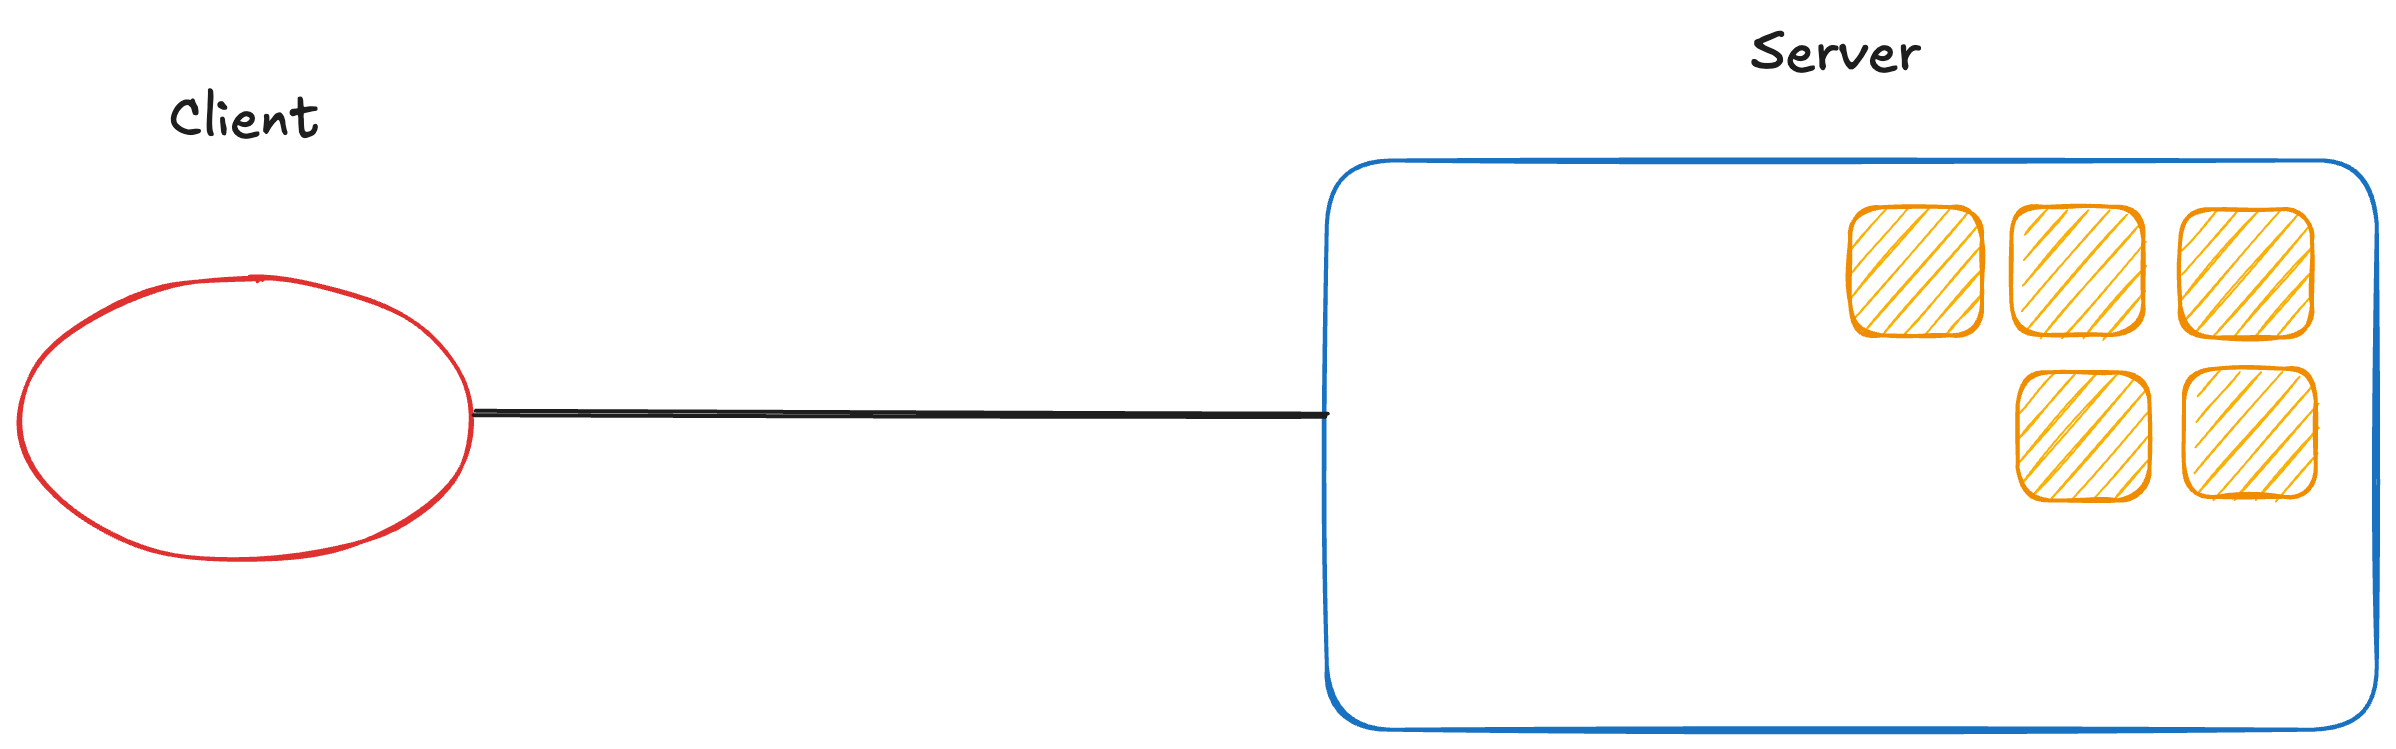
\includegraphics[width=0.8\textwidth, keepaspectratio]{figures/client-server.png}
\caption{Client-Server architectural style (own visualization inspired by Fielding \cite{fielding2000})}
\label{fig:client-server}
\end{figure}

In this architecture, clients initiate requests to servers, which manage resources. The server listens for incoming requests and either processes them by providing the requested resource or service or rejects them if they cannot be fulfilled. This separation of concerns allows client and server components to evolve independently \cite{sinha1992}.

\subsection{Client-Stateless-Server}

This principle requires that all communication between the parties be stateless, as illustrated in Figure ~\ref{fig:stateless}. This means that each request from the client must contain all the information necessary for the server to understand and process it\cite{MESBAH20082194}. As a result, the session state must be stored entirely on the client side.\cite[Section 3.4.1.]{fielding2000}

\begin{figure}[!h]
\centering
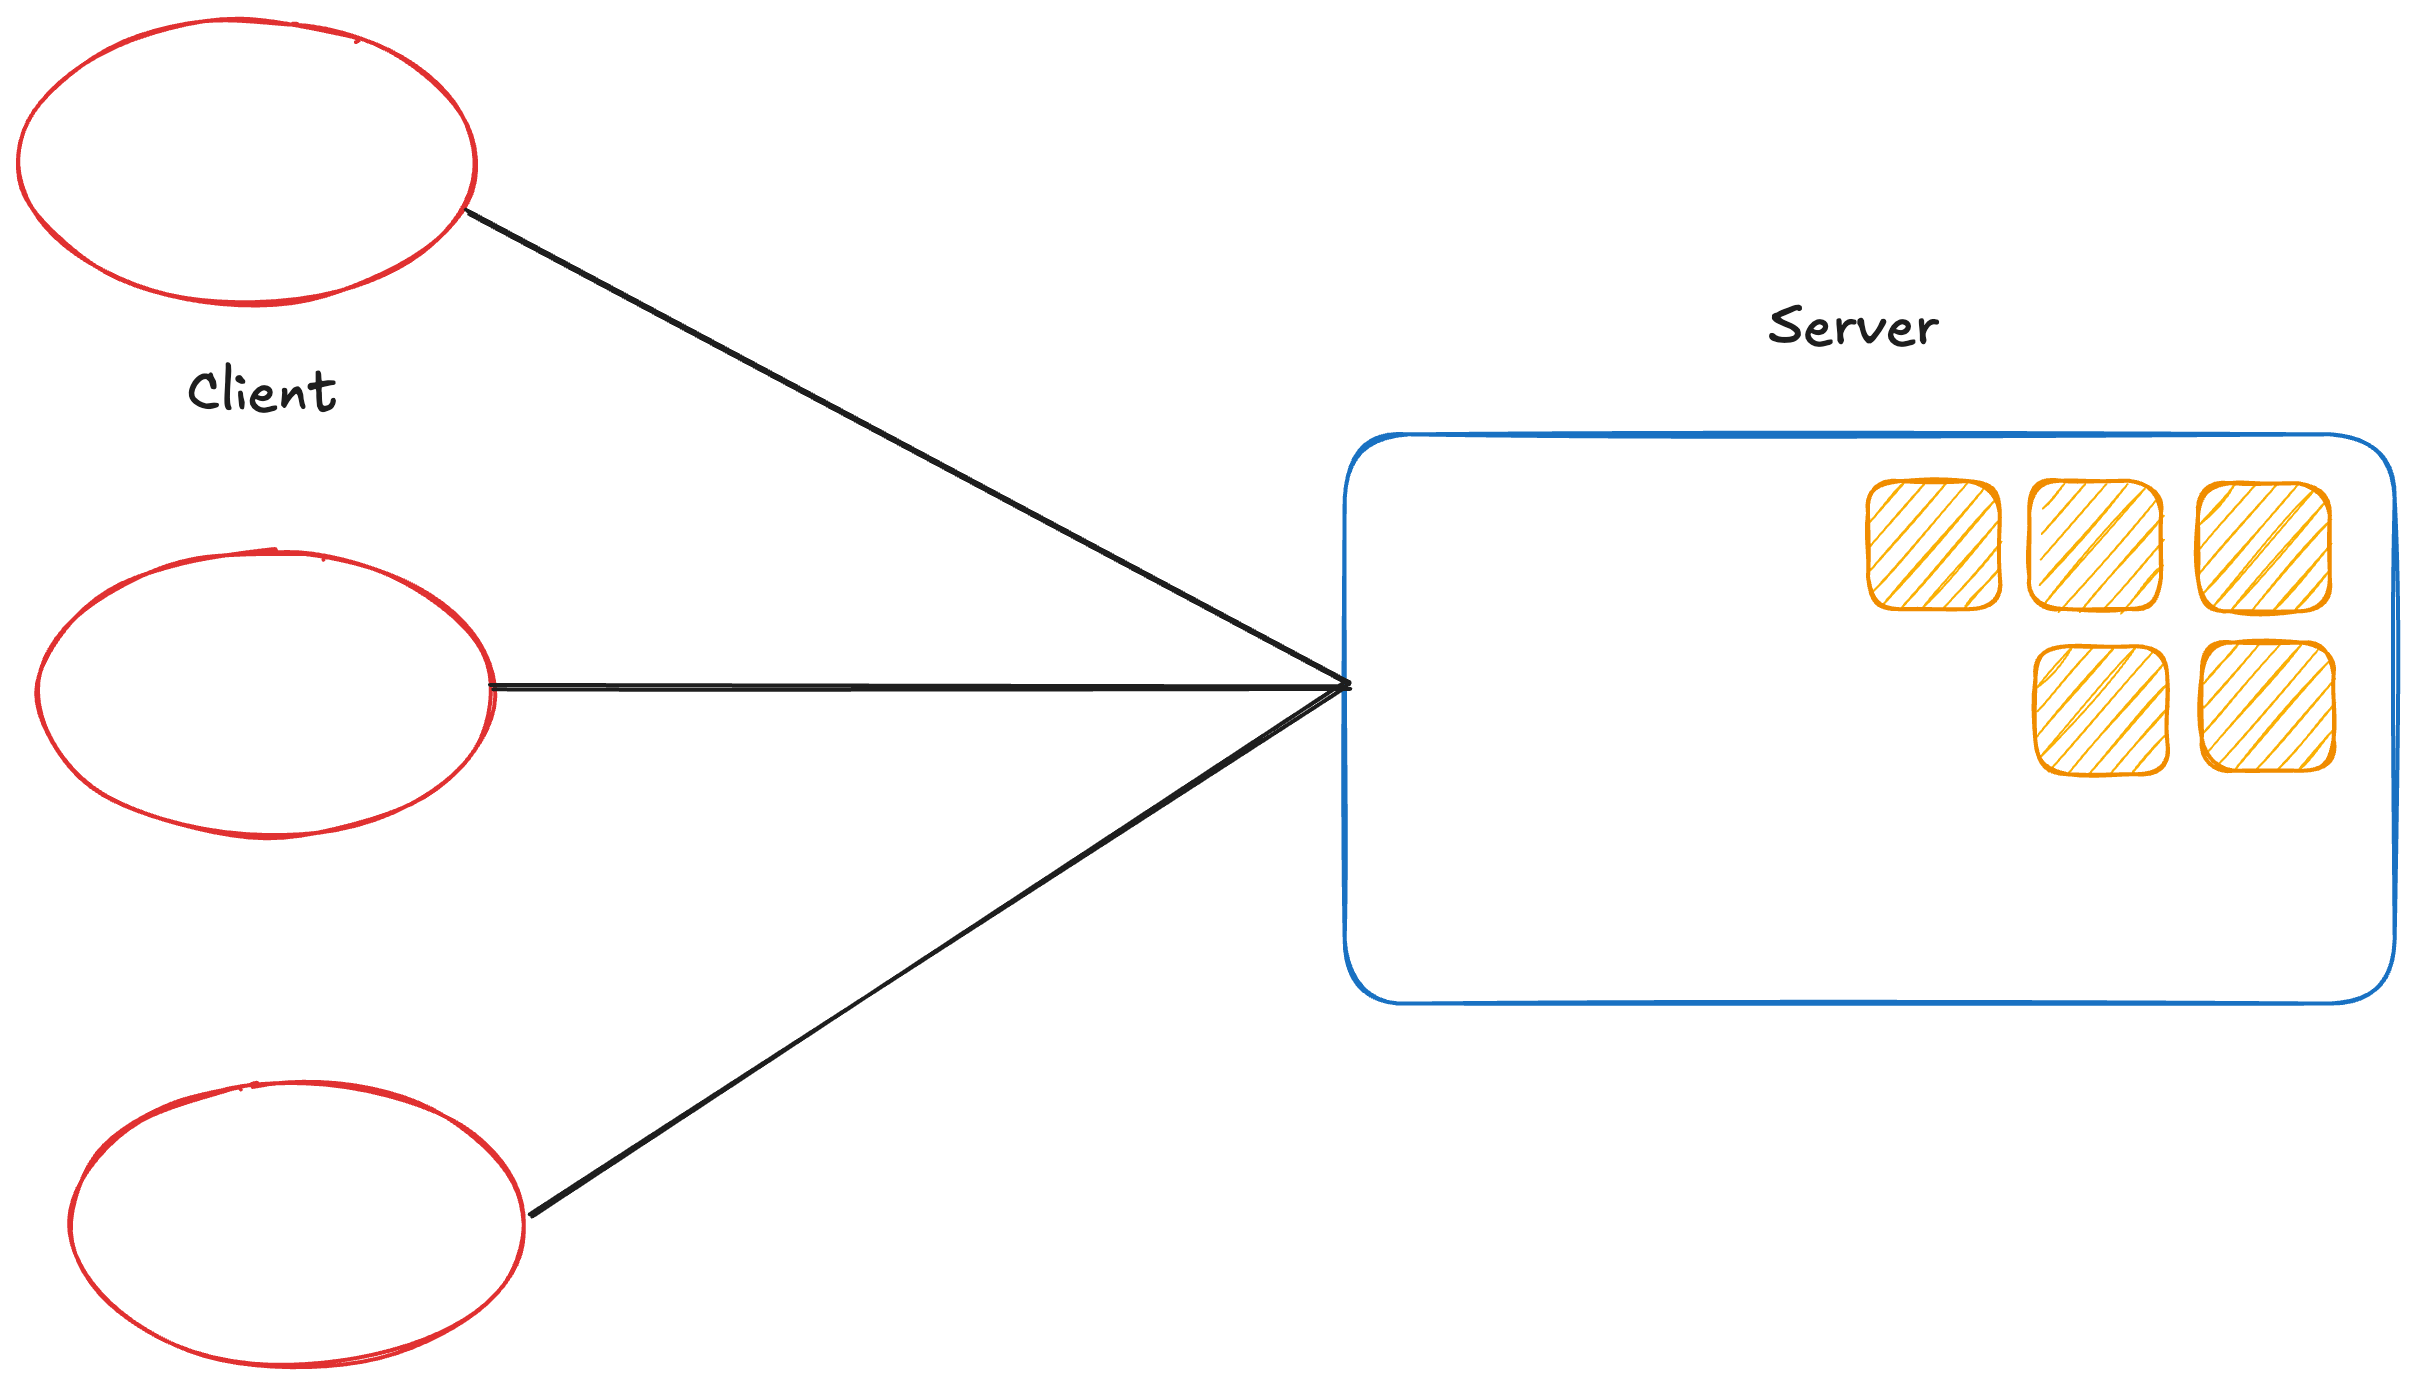
\includegraphics[width=0.8\textwidth, keepaspectratio]{figures/stateless.png}
\caption{Client-Stateless-Server (own visualization inspired by Fielding \cite{fielding2000})}
\label{fig:stateless}
\end{figure}

This constraint improves visibility, reliability, and scalability. However, it can decrease network performance due to the overhead of sending complete state information with each request \cite[Section 5.1.3]{fielding2000}.

\subsection{Cache}

The cacheable constraint requires that the response be labeled cacheable or non-cacheable. When labeled cacheable, the client has the right to use data later for a specified period.

\begin{figure}[!h]
\centering
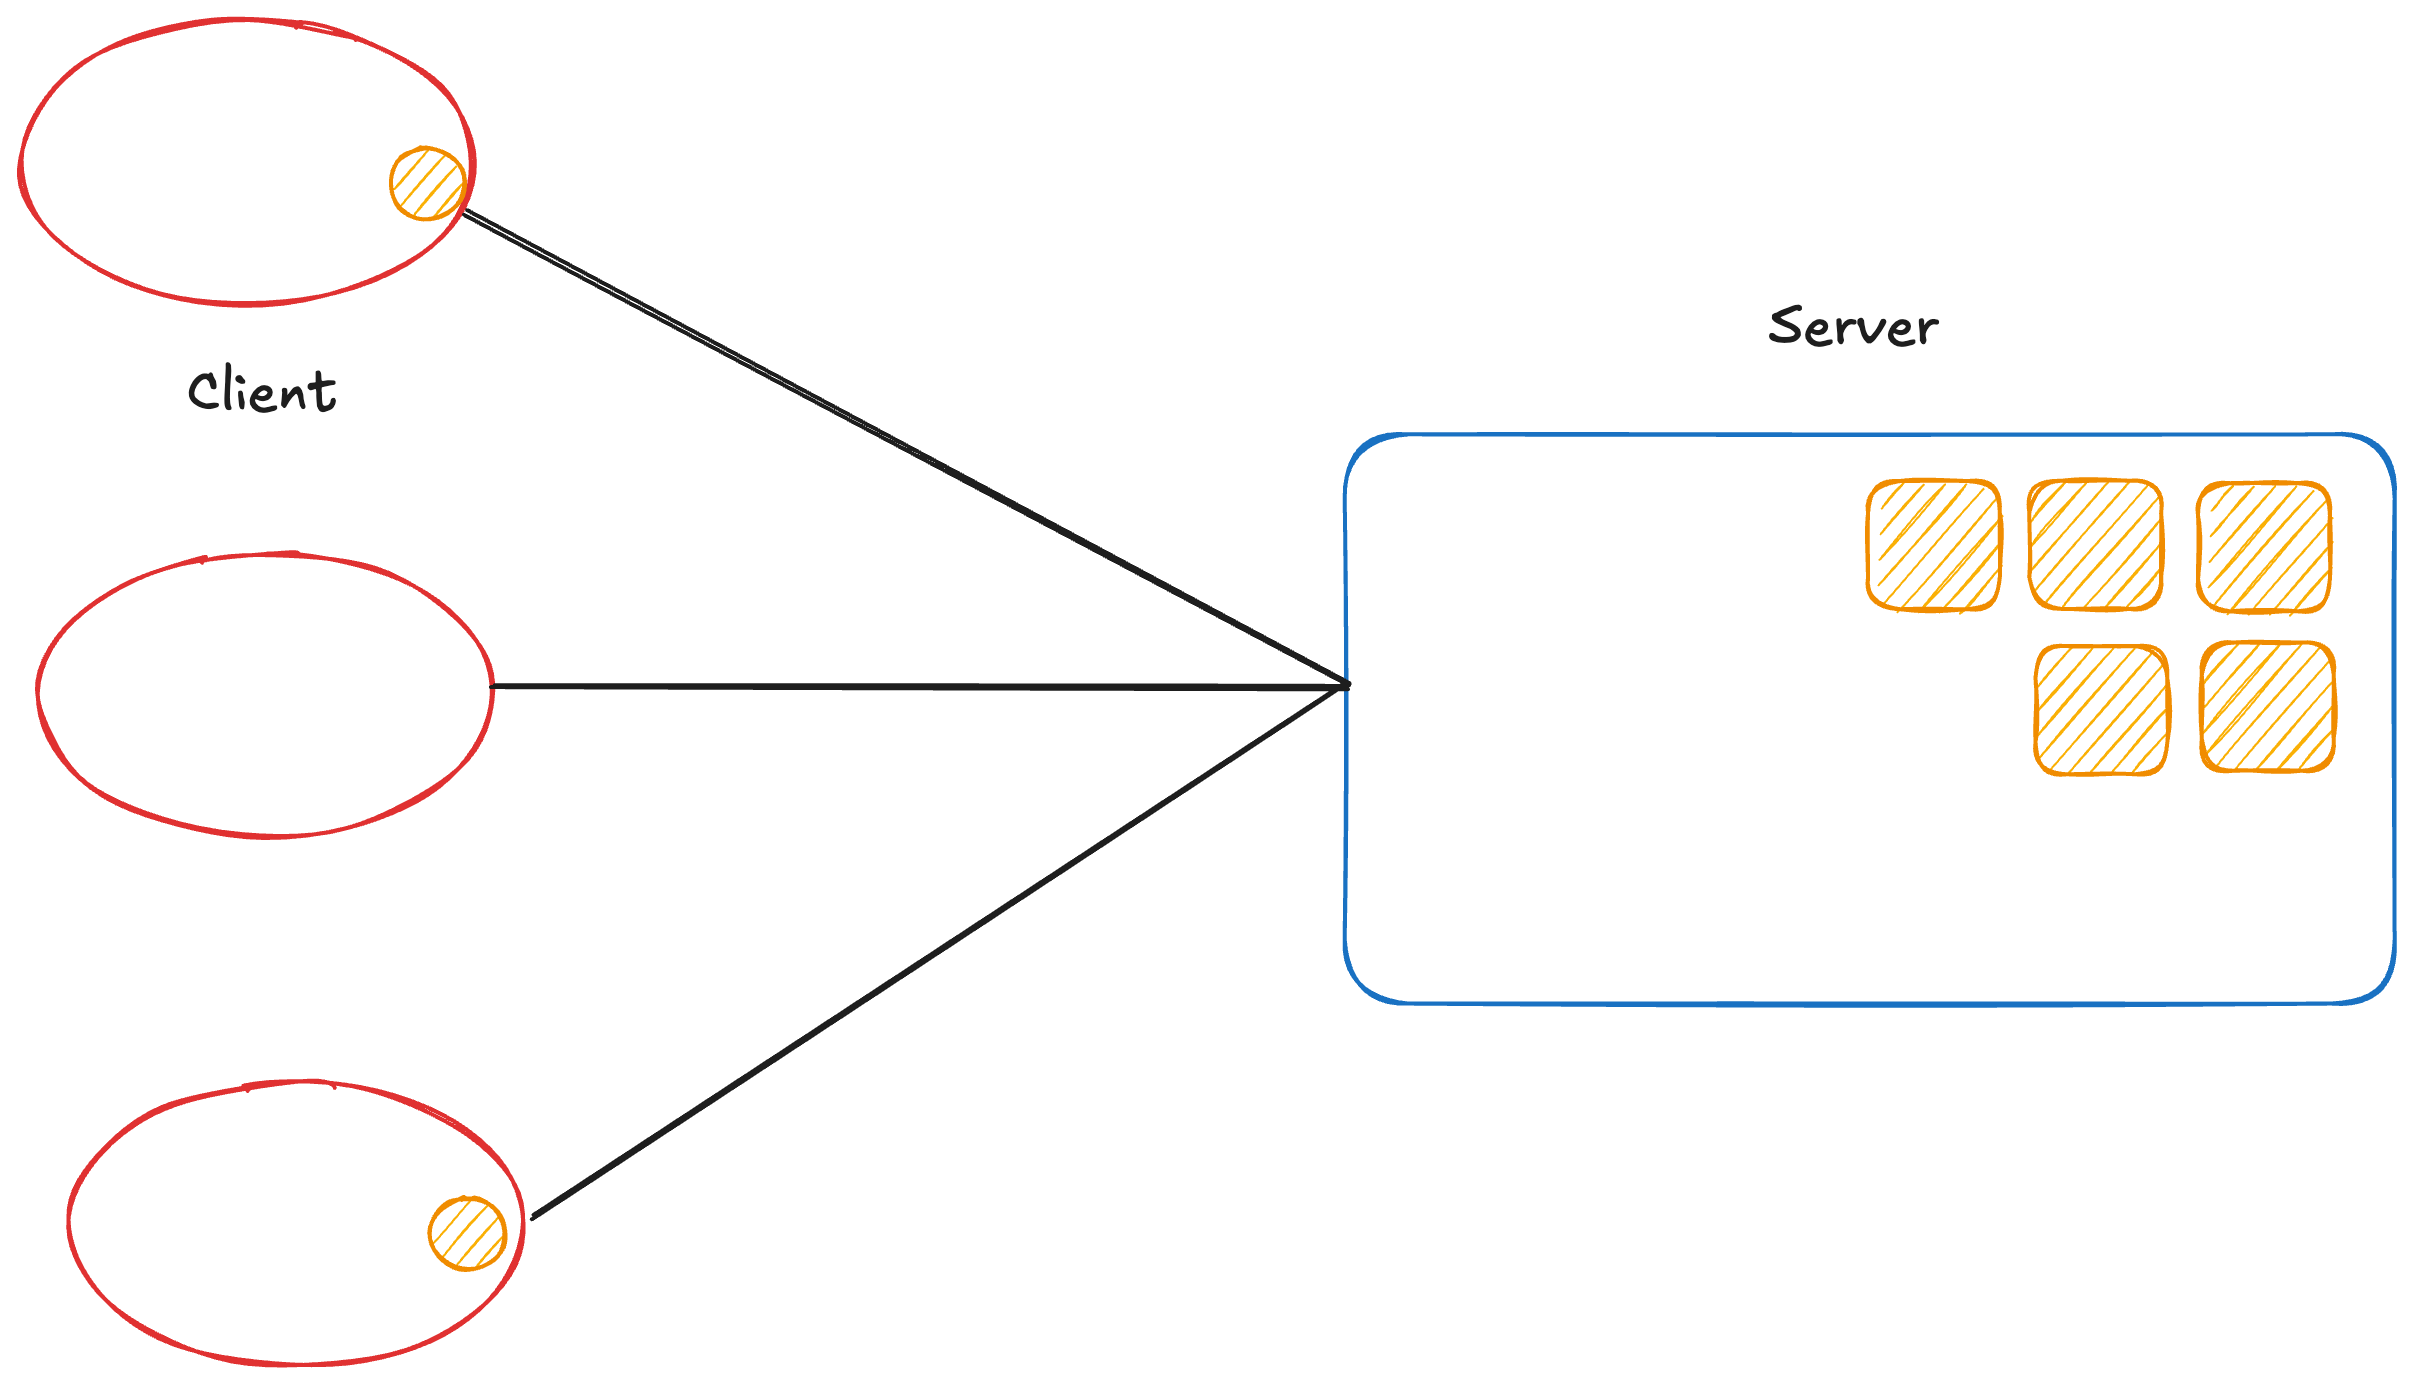
\includegraphics[width=0.8\textwidth, keepaspectratio]{figures/cache.png}
\caption{Cache (own visualization inspired by Fielding \cite{fielding2000})}
\label{fig:cache}
\end{figure}

\subsection{Uniform interface}
This principle says the REST services should ensure uniformity through these interface constraints:

\begin{itemize}
\item \textbf{Resource identification}: Each resource must be identified by a unique identifier URI. In practice, this is implemented by using URLs as identifiers.
\item \textbf{Resource manipulation}: Each resource should have a uniform representation on the server that the client can use to modify them.
\item \textbf{Self-descreptive messages}: Each request should contain enough information for the server to describe how to process them.
\item \textbf{HATEOAS}: The client application should dynamically drive all other resources and interactions using hyperlinks.
\end{itemize}

\begin{figure}[!h]
\centering
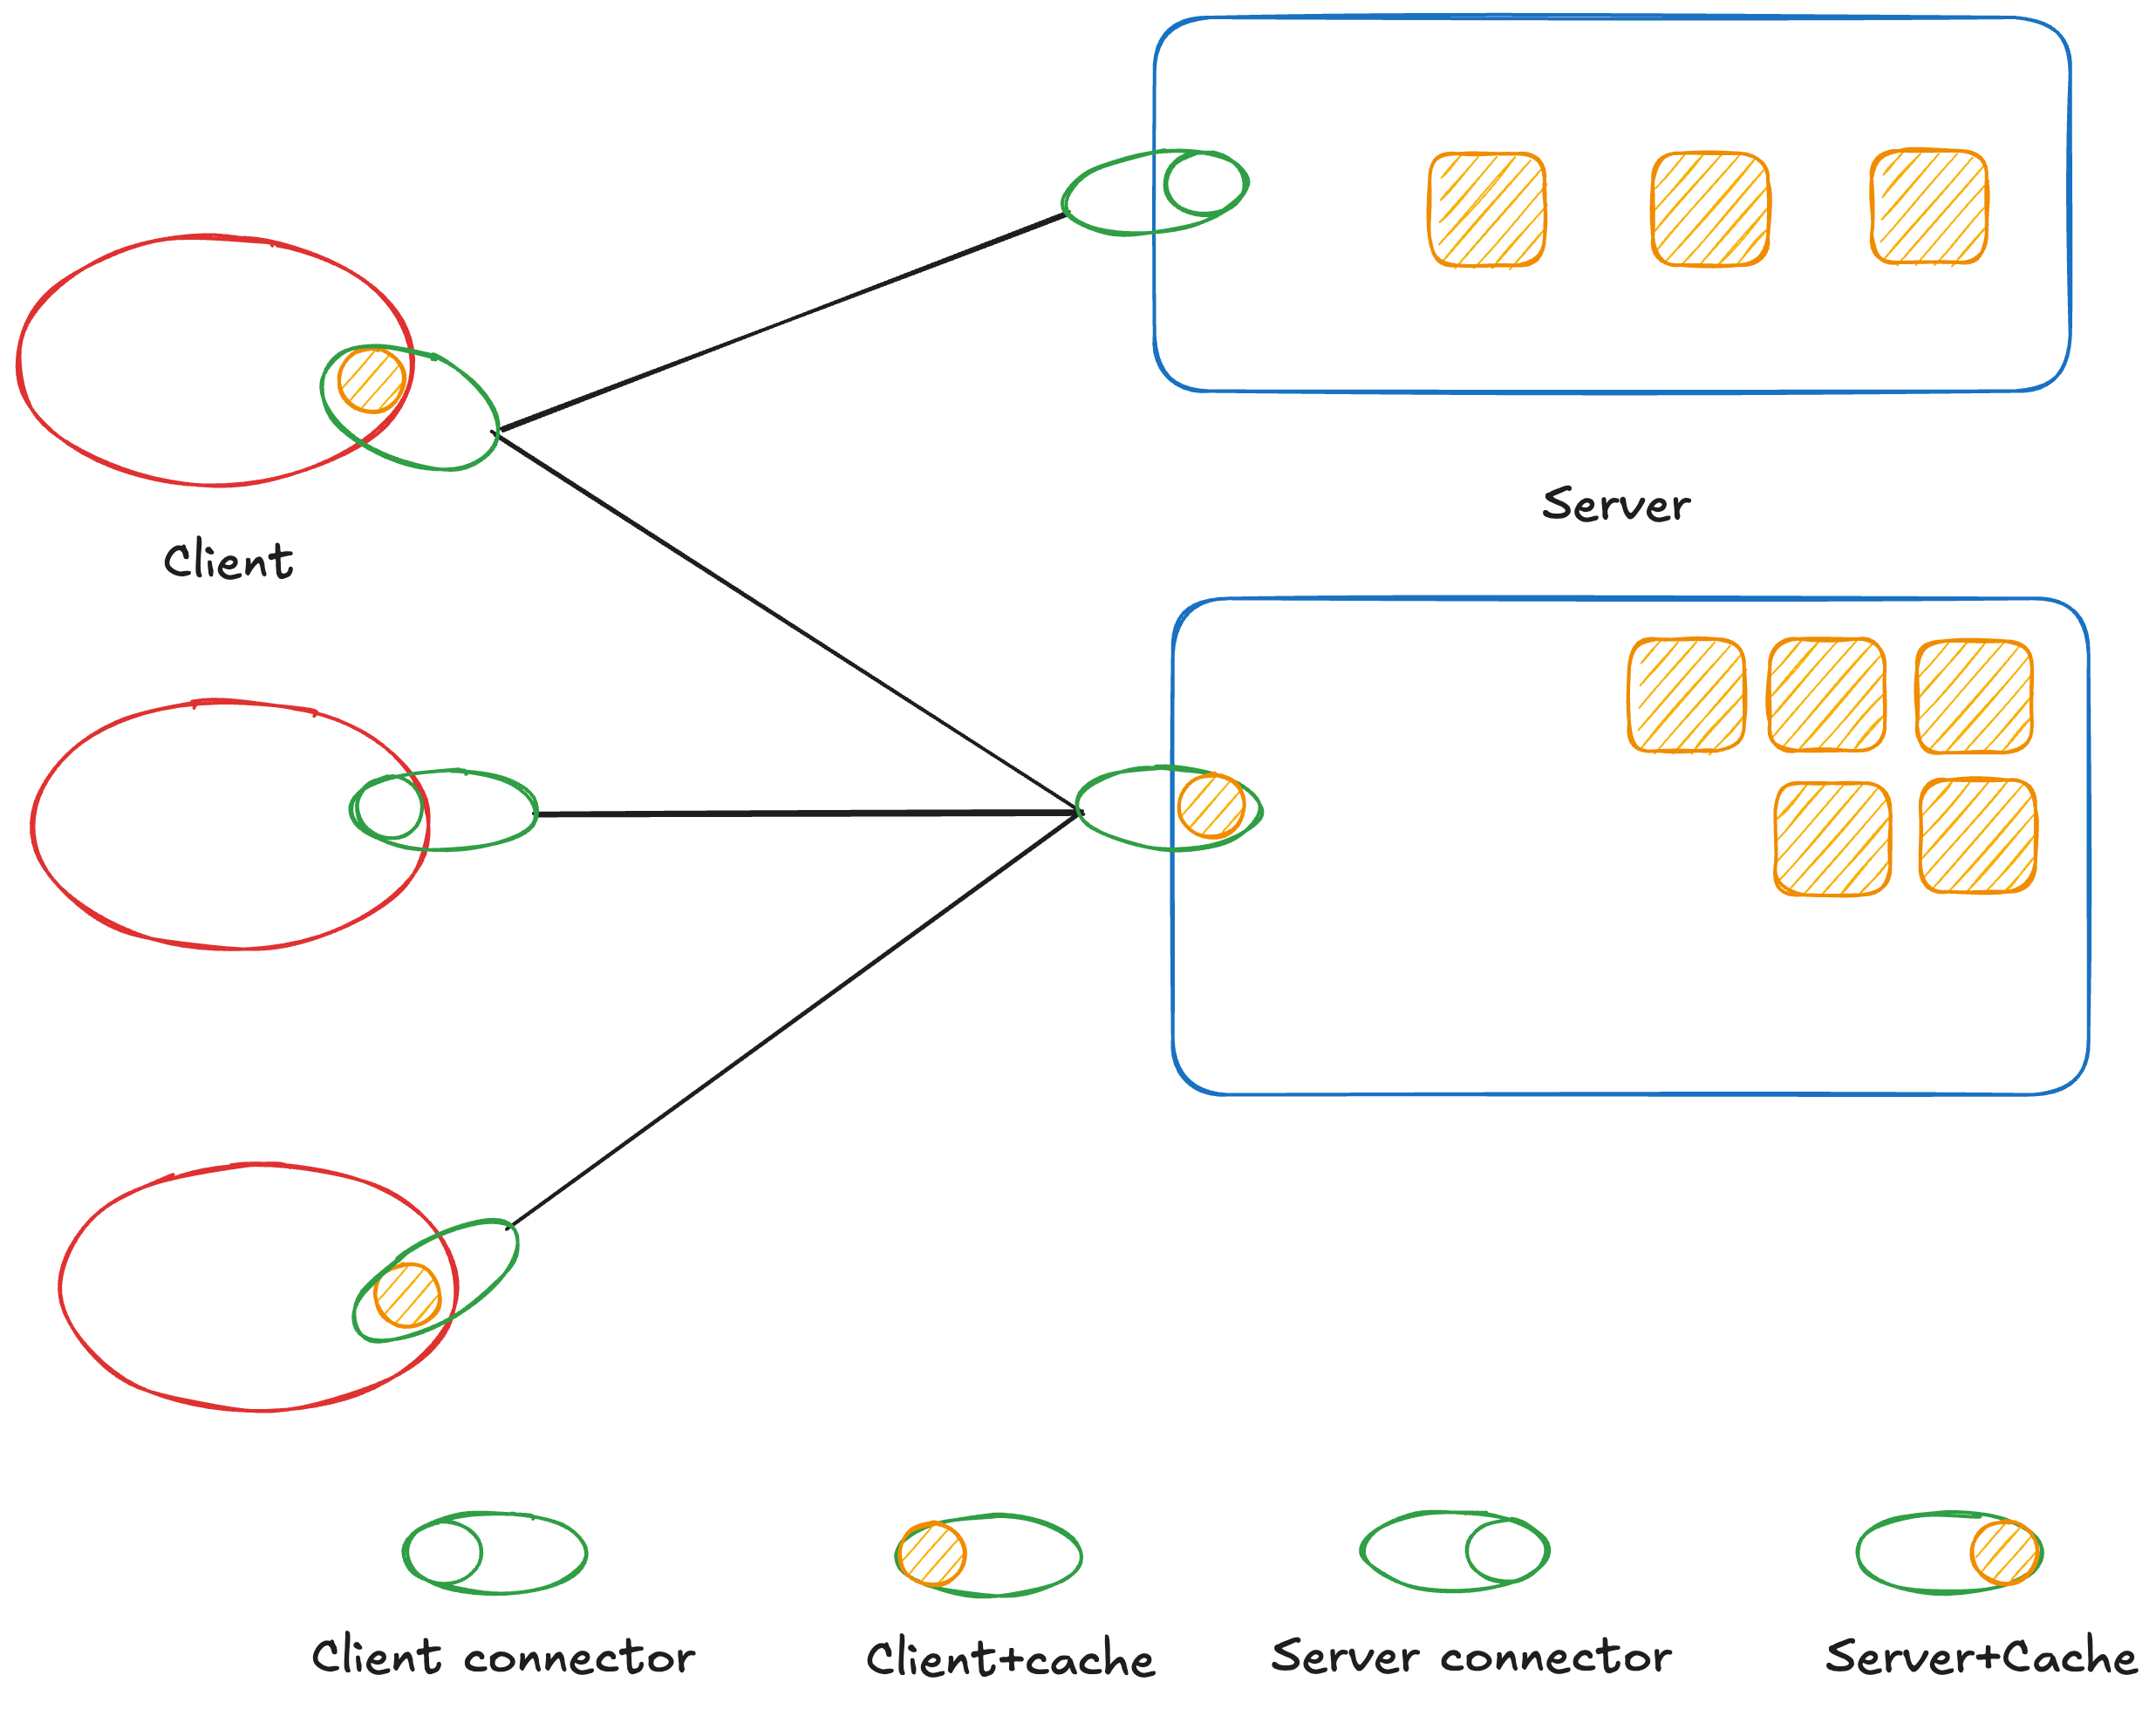
\includegraphics[width=0.8\textwidth, keepaspectratio]{figures/uniform-interface.png}
\caption{Uniform interface (own visualization inspired by Fielding \cite{fielding2000})}
\label{fig:uniform-interface}
\end{figure}

\subsubsection{HATEOAS}

HATEOAS is a small constraint that many people tend to forget. If we take the constraint strictly, most REST applications would not be REST applications. This is usually fine because most applications work differently than Fielding imagined in his dissertation back in the day. If we, a service, comply with it, all of its responses should contain the accessed data and the available actions as hyperlinks. The listing \ref{lst:hateoas} shows an example of a compliant response.

\begin{lstlisting}[caption=An HATEOAS response in JSON format,label=lst:hateoas, float]
{
  "accountId": "123456789",
  "accountName": "John Doe",
  "balance": 1500,
  "links": [
    {
      "rel": "self",
      "href": "http://examplebank.com/accounts/123456789",
      "method": "GET"
    },
    {
      "rel": "deposit",
      "href": "href": "http://examplebank.com/accounts/123456789/deposit",
      "method": "POST"
    },
    {
      "rel": "withdraw",
      "href": "href": "http://examplebank.com/accounts/withdraw",
      "method": "POST"
    }
  ]
}
\end{lstlisting}

One of the main ideas of HTMX is to be HATEOAS compliant. The website pages are generated dynamically on the server to contain the requested resource and all the actions available for the given resource. The server generates the page and adds HTMX requests to desired elements representing the actions.

\subsection{Layered System}

A layered system is another architectural style that allows splitting the service into different components placed in other layers. It will enable grouping, hiding, and defining behaviors between them. "Layers can be used to encapsulate legacy services and to protect new services from legacy clients" \cite{fielding2000}. These layers can also improve system scalability by enabling load balancing of the services. "The primary disadvantage of layered systems is that they add overhead and latency to the processing of data, reducing user-perceived performance" \cite{Clark1990ArchitecturalCF}. Figure \ref{fig:layered-system} shows the architecture of a complex, layered system.

\begin{figure}[!h]
\centering
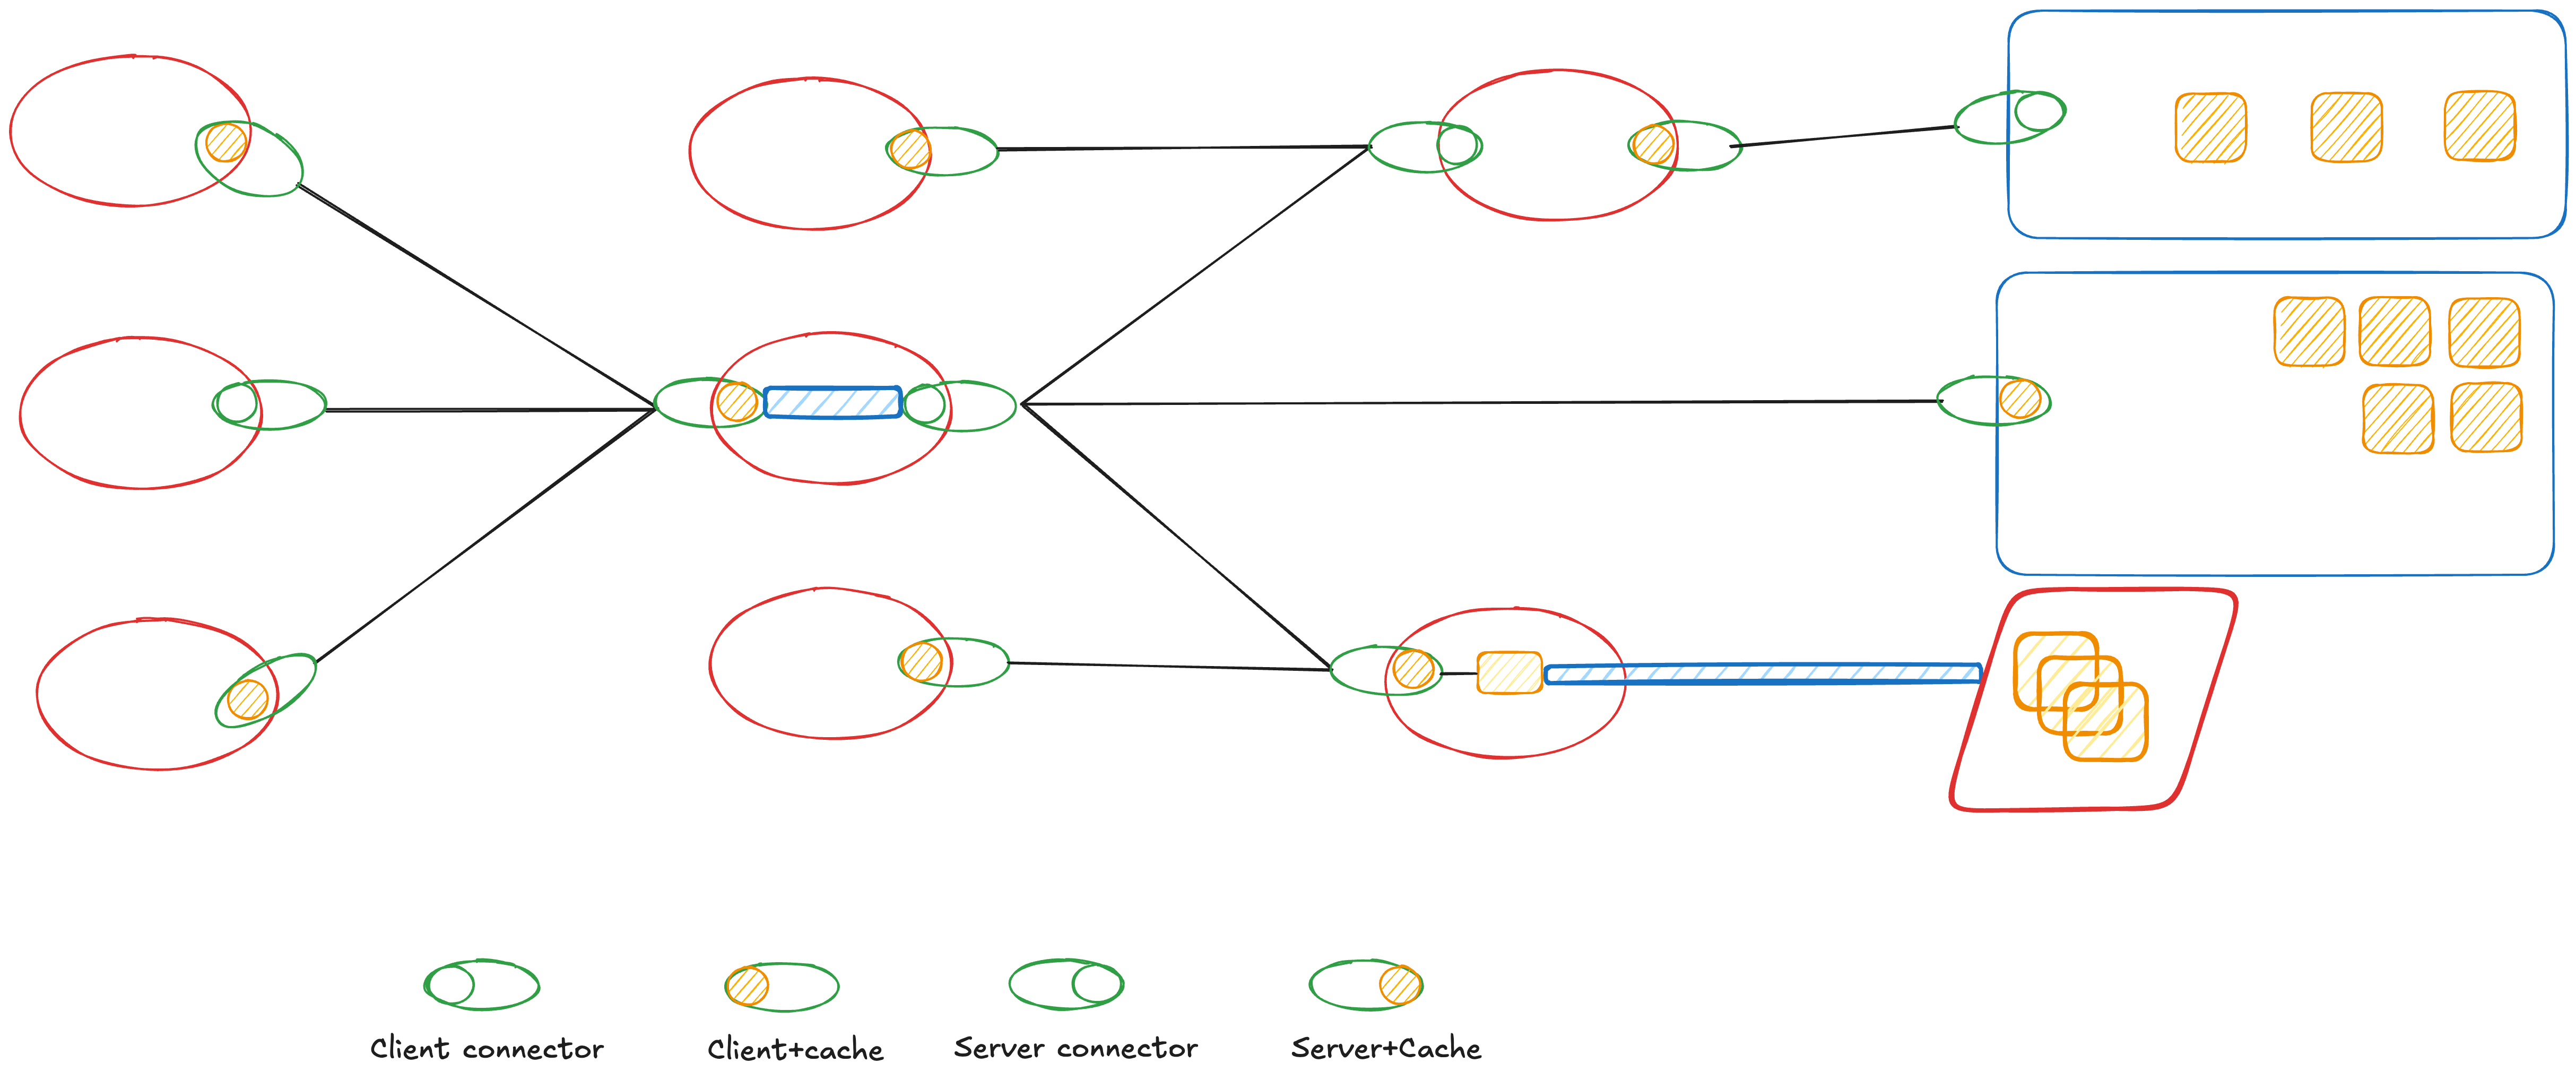
\includegraphics[width=0.8\textwidth, keepaspectratio]{figures/layered-system.png}
\caption{Layered System (own visualization inspired by Fielding \cite{fielding2000})}
\label{fig:layered-system}
\end{figure}

\subsection{Code-On-Demand}

Code-On-Demand is an optional constraint that the figure \ref{fig:code-on-demand} shows. It allows a client to extend its functionality by downloading and executing code as a script from a different source. "This simplifies clients by reducing the number of features required to be pre-implemented" \cite{fielding2000}. However, it is only an optional constraint because it reduces the overall visibility of a service.
 
\begin{figure}[!h]
\centering
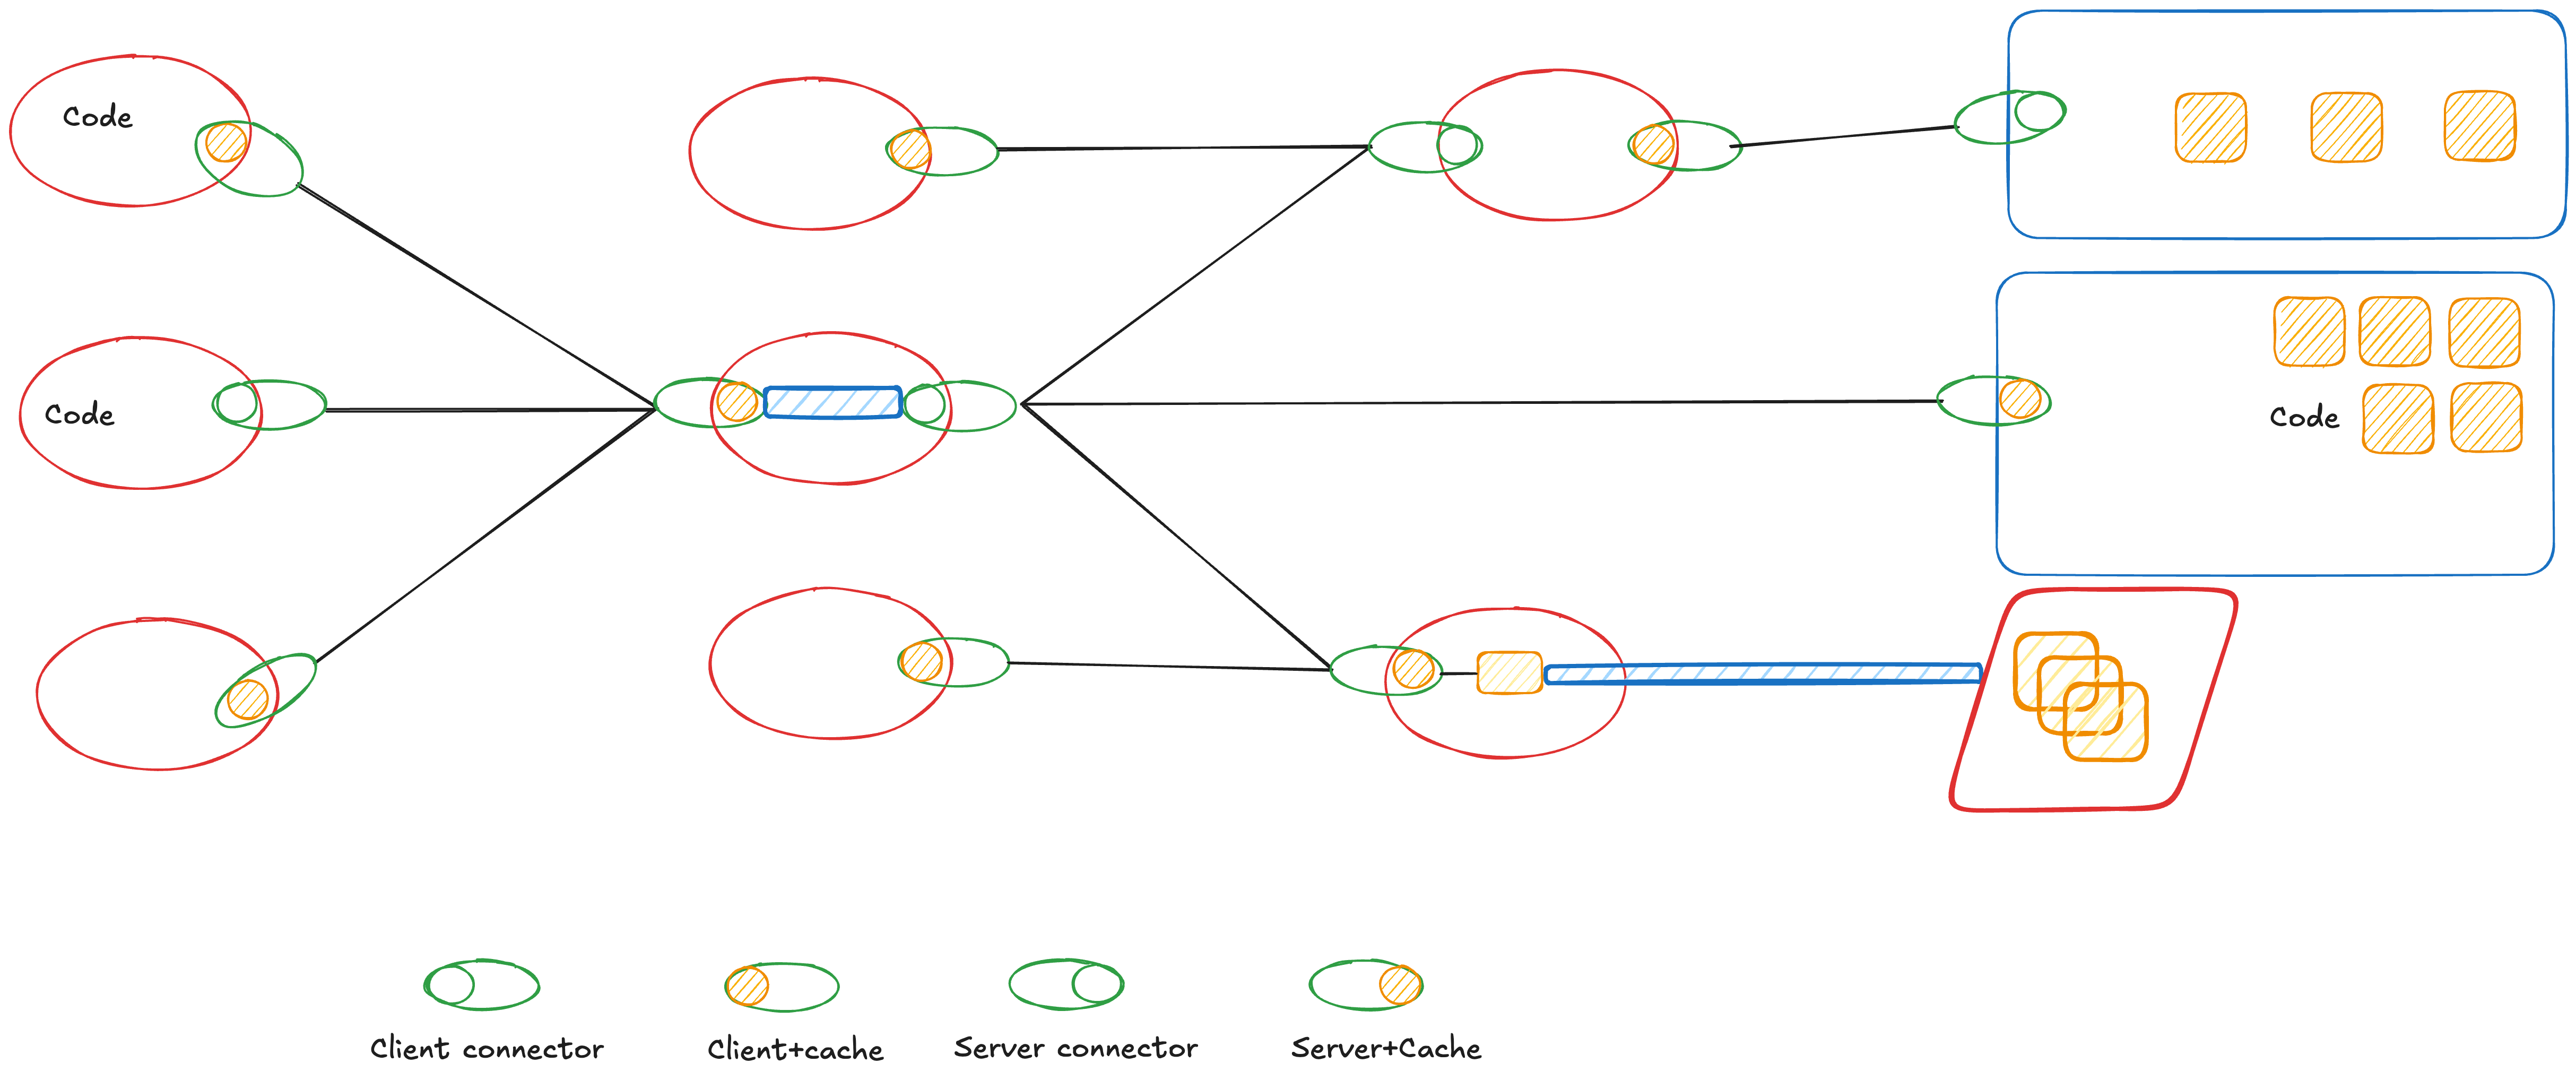
\includegraphics[width=0.8\textwidth, keepaspectratio]{figures/code-on-demand.png}
\caption{Code-On-Demand (own visualization inspired by Fielding \cite{fielding2000})}
\label{fig:code-on-demand}
\end{figure}